To evaluate our system, we perform quantitative experiments on camera pose estimation accuracy, and qualitatively analyse the obtained reconstructions.
%To evaluate the performance of our system we perform experiments that draw comparisons in terms of quantitative pose estimation and qualitative reconstruction quality and efficacy.
Firstly, the pose estimation accuracy is evaluated via a well-established SLAM evaluation benchmark~\cite{sturm12iros}.
We like to point out that % with the primary difference being that with
in traditional dense SLAM systems~\cite{Prisacariu2014,Niessner2013,Newcombe2011} -- for which the benchmark is often employed -- the entire contents of the visible scene are used for pose estimation, whereas in our system we rely only on points belonging to the object's surface.
Whilst more challenging, this implicitly allows us to track the camera wrt. the object regardless of which of the two is subject to motion.
Then, qualitative comparisons are drawn between the reconstructions attained by our system, and those of the method described in \cite{Ren2013}.
We evaluate our system on multiple frame sequences depicting objects of different sizes. %; some with the object moving wrt. a fixed camera, others with the sensor in motion.% in the case of qualitative evaluation.

%\vspace{-.7\baselineskip}

\subsection{Pose Estimation Quality}
In this section we present quantitative results of our systems' %ability to maintain tracking
robustness in estimating the camera motion, by performing tracking against the reconstruction of a single object, instead of the whole scene.
The trajectories estimated by our system demonstrate low tracking drift. % and a robustness to loop closure events.
We perform such evaluation on two sequences of the RGB-D SLAM Dataset~\cite{sturm12iros} depicting static objects observed by a moving camera.
Tracking is performed using purely geometric clues, by matching the current depth frame with a rendering of the reconstructed object using a projective ICP tracking approach~\cite{Kahler2016}.
%, as such the evaluation is of camera pose estimation when tracking an object.
%By tracking the sensor pose against a subset of the observed scene 
%At this point it should be highlighted that our system is at a disadvantage when compared to dense SLAM systems that utilise the entire scene geometry for pose optimisation.

%In the following experiments, tracking is performed using only geometry cues from the rendered object models and the instantaneous depth frame.\\

%The tracking accuracy is evaluated via the Absolute Trajectory Error (ATE) metric, as outlined in \cite{sturm12iros}, and is summarised in Table~\ref{ateTable}.

\iffalse
\begin{table}[!t]
	{
        \footnotesize
		\begin{center}
			\begin{tabular}{l@{\hskip 1cm} c}
				\emph{Sequence Name} & \emph{ATE (m)}\\
				\midrule
				\textsf{freiburg3\_cabinet} & 0.078 \\ %0.077903
				\textsf{freiburg3\_teddy}   & 0.031 \\ %0.030596
			\end{tabular}
		\end{center}
	}
	\caption{Absolute Trajectory Error (ATE) results (lower is better) achieved by our approach.}
	\label{ateTable}
\end{table}
\fi

\begin{figure}[!t]
	\centering
	\begin{tabular}{cc}
		\fbox{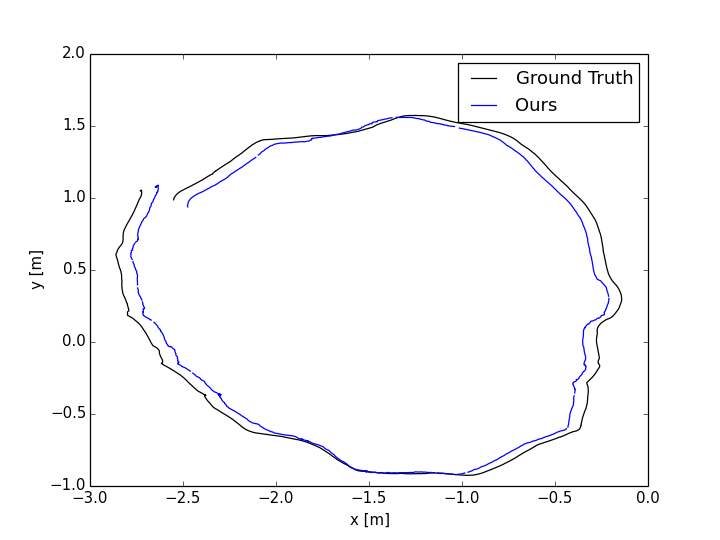
\includegraphics[width=0.25\textwidth]{results/rgbd_dataset_freiburg3_cabinet.png}} \\[2ex] \fbox{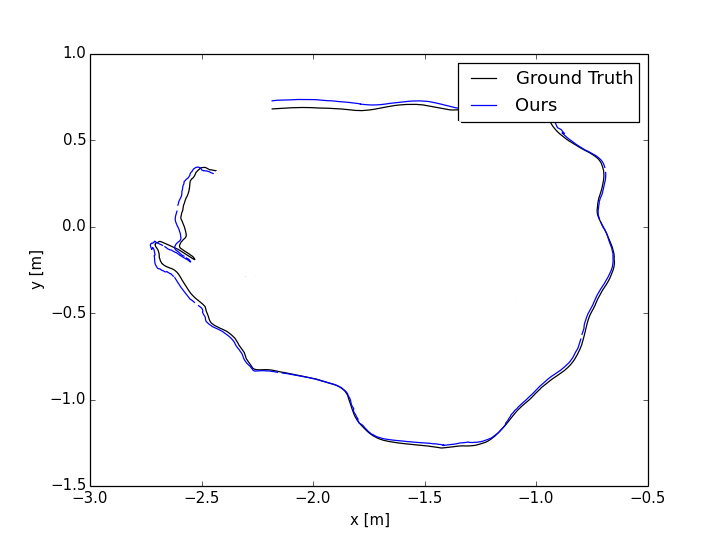
\includegraphics[width=0.25\textwidth]{results/rgbd_dataset_freiburg3_teddy.png}}
	\end{tabular}
	\caption{
        Comparison of the estimated camera trajectory with the ground truth for
		\textbf{(L)}~\textit{freiburg3\_cabinet} (final ATE:~$0.078m$), and
		\textbf{(R)}~\textit{freiburg3\_teddy} (final ATE:~$0.031m$).
	}
\label{fig:tumTrajectories}
\end{figure}

At this point, it should be highlighted that our proposed system is at a disadvantage when compared to dense SLAM systems that utilise the entire scene geometry for pose optimisation, since we track the sensor pose against a subset of the observed scene.
Nevertheless, as shown by the results in Figure~\ref{fig:tumTrajectories}, our system is able to robustly estimate trajectories close to the ground truth whilst using only the objects' geometric appearance.
Quantitatively, the tracking accuracy is evaluated via the Absolute Trajectory Error (ATE) metric, as outlined by \cite{sturm12iros}.
The cabinet reconstructed in the \textit{freiburg3\_cabinet} sequence is lacking in geometric features, as the object is mostly planar,
%It can be seen that there is a
and the small deficit in tracking quality is mostly due to this factor.
However, our system remains able to estimate a fairly accurate trajectory. 
In the \textit{freiburg3\_teddy} sequence we determine a trajectory very close to the ground truth.
Improvement over the accuracy in \textit{freiburg3\_cabinet} is due to the wider availability of geometrical features, such as curves in the teddy's body and head.

\subsection{Qualitative Reconstruction Quality}
In this section we present a qualitative comparison of our method vs. the approach by Ren et~al.~\cite{Ren2013} in the reconstruction of closed object models. %by relying on a variety of sequences and demonstrating efficacy over \cite{Ren2013} in this regard.
Each sequence is run through both systems; to evaluate the obtained results we regularly take snapshots of the reconstruction, in the case of our system, and the level set evolutions, in the case of \cite{Ren2013}.
Such snapshots are captured after each quarter of a sequence has been processed. %quarterly intervals of the systems run time through the sequence.

\begin{figure}[!t]
	\centering
	\begin{tabular}{cc}
		\fbox{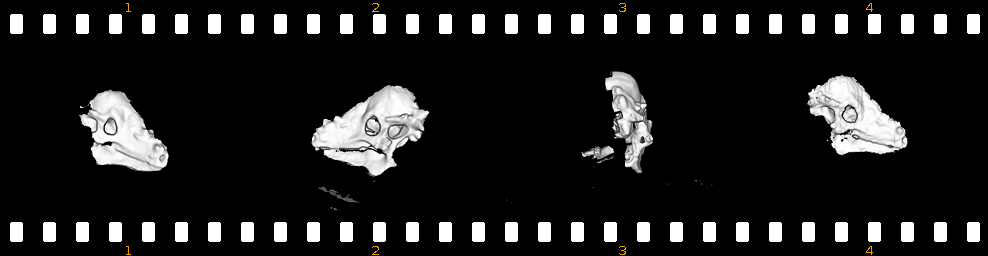
\includegraphics[width=0.45\textwidth]{filmstrips/dino.png}} \\ [2ex]
		\fbox{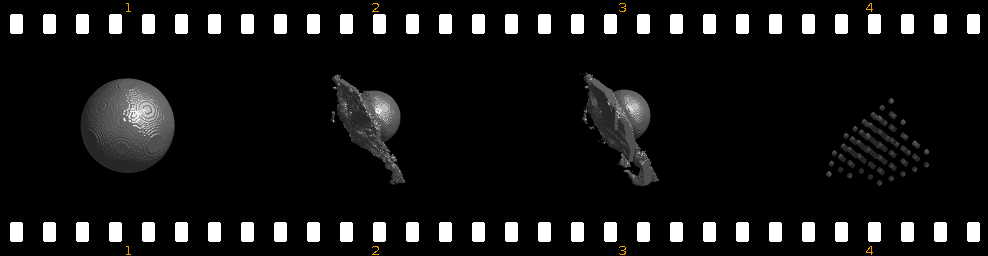
\includegraphics[width=0.45\textwidth]{filmstrips/dino_s3d_large.png}}
	\end{tabular}
	\caption{
        Quarterly interval snapshots of the Dinosaur Head reconstruction using \textbf{(L)} our method, and \textbf{(R)} the one proposed by Ren et~al.~\cite{Ren2013}.
	}
	\label{fig:dinoComparison}
\end{figure}

\begin{figure*}[!t]
	\centering
	\begin{tabular}{ccc}
		\fbox{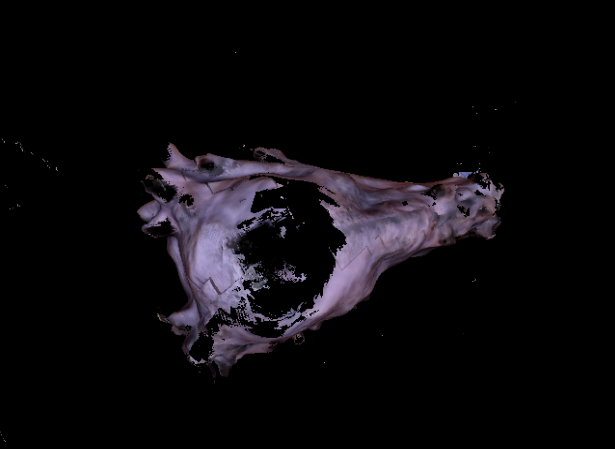
\includegraphics[width=0.2\textwidth]{screenshots/dino_colour_top.PNG}}&
		\fbox{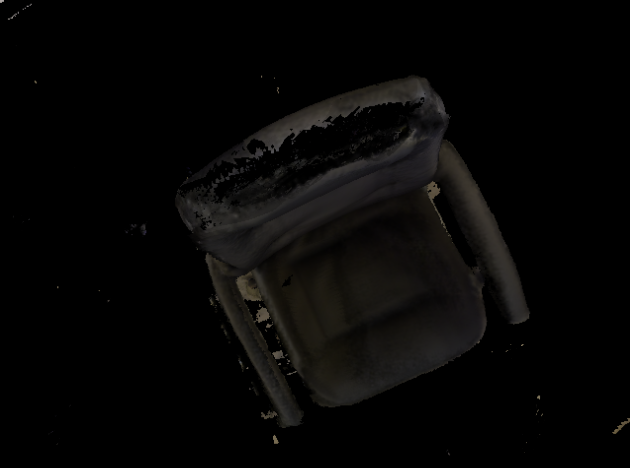
\includegraphics[width=0.2\textwidth]{screenshots/chair_colour_top.PNG}}&
		\fbox{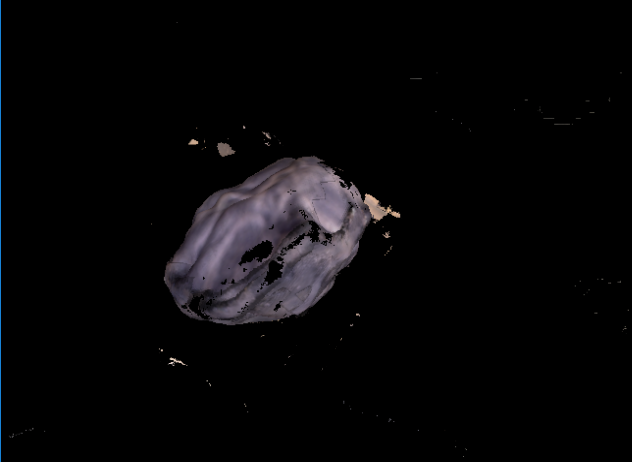
\includegraphics[width=0.2\textwidth]{screenshots/rock_colour_top.PNG}}
	\end{tabular}
	\caption{
		Closed reconstructions of \textbf{(L)} a Dinosaur Head,
		\textbf{(M)} a Chair, and
		\textbf{(R)} a Rock.
	}
	\label{fig:top_shots}
%	\vspace{-\baselineskip}
\end{figure*}

As depicted in Figure~\ref{fig:dinoComparison}, our method is able to successfully reconstruct the Dinosaur Head, whereas the approach by Ren~et~al. fails to converge towards a feasible shape.
In addition, Figure~\ref{fig:top_shots} demonstrates that our system is able to generate consistent models (unaffected by camera tracking drift) for a variety of sequences containing several loop closures.
Failure of the competing method %of Ren et al
is also apparent for other sequences evaluated in this work, all presenting failure cases analogous to Figure~\ref{fig:dinoComparison}b. % to converge to a correct shape.
Such examples will be presented in the supplementary materials.
%The supplementary materials to this work demonstrate our efficacy vs that of Ren et al \cite{Ren2013}.\\

The object reconstructions depicted in Figure~\ref{fig:demo} have been obtained from sequences in which a camera was moved in a loop around each object in order to generate a closed model.

%As can be seen from the top down views of Figure \ref{fig:top_shots}, our system is capable of producing closed models, unaffected by tracking drift and loop closure events.